\documentclass{article}



\usepackage{arxiv}

\usepackage[utf8]{inputenc} % allow utf-8 input
\usepackage[T1]{fontenc}    % use 8-bit T1 fonts
\usepackage{hyperref}       % hyperlinks
\usepackage{url}            % simple URL typesetting
\usepackage{booktabs}       % professional-quality tables
\usepackage{amsfonts}       % blackboard math symbols
\usepackage{nicefrac}       % compact symbols for 1/2, etc.
\usepackage{microtype}      % microtypography
\usepackage{lipsum}		% Can be removed after putting your text content
\usepackage{graphicx}
\usepackage{natbib}
\usepackage{doi}



\title{Face Mask Detection and Attack with One Pixel Change}

%\date{September 9, 1985}	% Here you can change the date presented in the paper title
%\date{} 					% Or removing it

\author{ Yang Hu \\
	\texttt{yanghu@live.unc.edu} \\
	%% examples of more authors
	\And
	Kangda Wei \\
	\texttt{kangda@live.unc.edu} \\
	\And
	Yuchen Bai \\
	\texttt{yuchencc@email.unc.edu} \\
}

% Uncomment to remove the date
%\date{}

%%% Add PDF metadata to help others organize their library
%%% Once the PDF is generated, you can check the metadata with
%%% $ pdfinfo template.pdf
\hypersetup{
pdftitle={COMP 562 Final Project},
pdfsubject={q-bio.NC, q-bio.QM},
pdfauthor={Yang Hu, Kangda Wei, Yuchen Bai},
}

\begin{document}
\maketitle


\section{Introduction}
The pandemic COVID-19 has changed the world in 2020 and it continues its impact in 2021. People are required to wear medical masks and keep social distance in order to mitigate propagation of such airborne disease. There is thus an increasing demand on medical mask detection in public places, such as hospitals, railway stations, and shopping malls, to remind people who don't wear masks. Medical mask detection with AI not only saves labors to check, but also minimizes unnecessary contact between pedestrians and checkers. Our research paper thus try to use MTCNN and Residual Neural Network (ResNet) to implement a model to detect whether human in a picture properly wear medical masks.we further our research to examine one pixel attack to our detection model trained in the previous stage. we implement the one pixel attack using differential evolution algorithm to find an one-pixel perturbation that changes the detection result of a image classification model. The code for the project is listed on: https://github.com/hmumixaM/562project.
%Additionally, inspired by the research that wearing T-shirt with certain pattern can make human invisible to facial recognition neural networks \cite{tshirt}, we further our research to examine one pixel attacks to our detection model trained in the previous stage. With the guide of Su's paper \cite{onepixel}, we implement the one pixel attack using differential evolution algorithm to find an one-pixel perturbation that changes the detection result of a image classification model. The code for the project is listed on: https://github.com/hmumixaM/562project. %

\subsection{Related Works}
Because of current pandemic situation around the world, more published research papers are related to the face mask detection. In general, the mask detection mainly consists of 2 parts: face detection and classification. However, we further explore the one-pixel attack by using our Face masks data set. The one-pixel attack aims to change the classification of the targeted image. Combining one-pixel attack and face mask detection, we could explore the potential possibility of misdirecting face mask detection by only one-pixel change. In other words, this research result would help the future researcher to find the loophole and improve the system.

In research \cite{tshirt}, it mainly discussed how wearing T-shirt with certain pattern can make human invisible to facial recognition neural networks. In \cite{onepixel}, it analyzed the extreme case that  out put of deep neural networks altered by one-pixel modification.

In the research\cite{facemaskdetect}, the authors applied Single Shot Multibox Detector as face detector and MobilenetV2 as classifier to perform the face mask detection. Their face mask detection system achieved 92\% accuracy.  In the research\cite{Yolo-v2}, the authors used YOLO-v2 with ResNet-50 model and carried out 81\% precision percentage on facemask detection.



\section{Mask Detection}
\subsection{Dataset}
We use the Face Mask Detection Dataset on Kaggle to train our model \cite{kaggle}. The dataset is structured to have 6024 images and corresponding annotations. Each image may contain more than one face, and its annotation explicates number of faces, bound of each face, and whether mask is wore. 


The dataset is prepossessed before feed into our model. First, there are different kinds of masks specified in the dataset. We classify them into two categories—"face\_with\_mask" and "face\_without\_mask"—to only determine whether a face wear a mask. Furthermore, we use the module MTCNN for Keras to find bound of faces in each picture. The images are then cropped and resized into 50x50 pixels images with only faces based on the detection result from MTCNN. 

\begin{figure}[h]
	\centering
    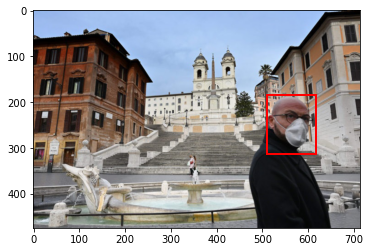
\includegraphics[width=8cm]{download-1.png}
    \caption{Find Bound of Faces by MTCNN.}
\end{figure}

\subsection{Model}
We applied residual neural network, which is widely used in image recognition, to build the following model. We use 80\% of cropped faces to train the model, and leave the following 20\% to faces to test on the model. Moreover, we use the Adam optimizer in trading which is computationally efficient and invariant to diagonal re-scale of the gradients \cite{onepixel}. 

\begin{figure}[h]
	\centering
    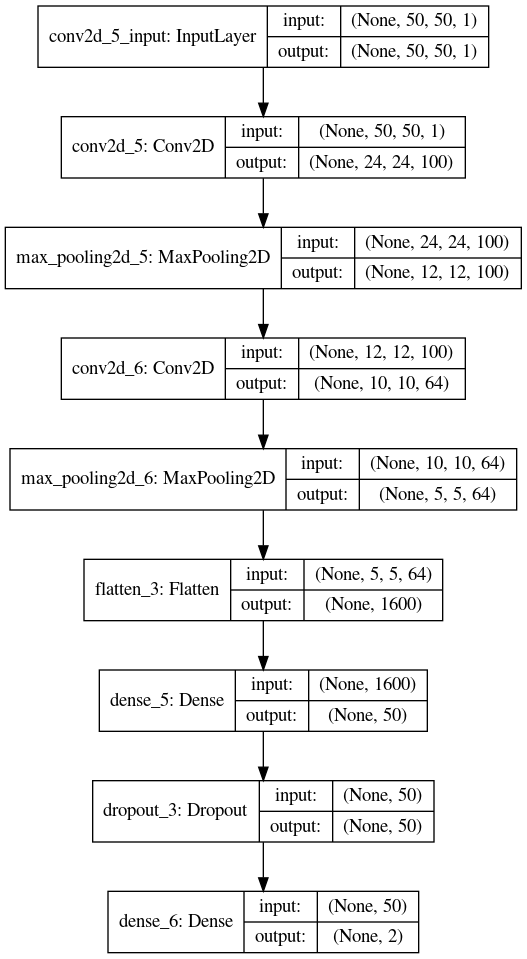
\includegraphics[width=6cm]{model.png}
    \caption{Visualization of the ResNet Model.}
\end{figure}


\subsection{Result}
The trained model has 94.20\% accuracy on determining whether a face wear the mask or not. On the average, the face mask detection system spends 10 seconds on each image.

\section{One Pixel Attack}
\subsection{Summary}
In order to perform the attack, we use an Evolutionary Algorithm called Differential Evolution (DE) that iteratively generate adversarial images, which are acquired by selecting a pixel and changing its color, to try to minimize the confidence of the neural network's classification. For a specific image, we first generate several adversarial images by picking and modifying a random pixel. We then run the images through the neural network to get the probability distribution of the classification. Next, we combine the positions and colors of the previous images' random pixels to generate new adversarial images and run through the neural network. If the newly generated pixels reduced the confidence of the network from previous step, we treat them as the current optimal solutions. We acquire the final answer by repeating the former steps and return the adversarial image on the last iteration that decrease the confidence of the network the most. A successful attack will have an adversarial image whose confidence of the correct category would be reduced so much that a new category now has the highest classification confidence. \cite{github}
\begin{figure}[h]
	\centering
    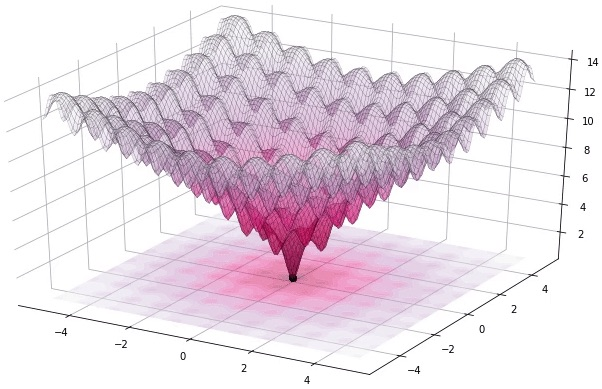
\includegraphics[width=8cm]{Ackley.jpg}
    \caption{Visualization of Differential Evolution.}
\end{figure}


\subsection{Result}
The following selected examples show the feasibility of the one pixel attack. A perturbation of one pixel can totally invert the classification result provided by ResNet. However, the differential evolution algorithm cannot achieve significant attack success rate, because our ResNet model doesn't provide continuous confidence level for the algorithm to fit. Therefore, only about 1.77\% of pictures are successfully attacked. 

\begin{figure}[h]
	\centering
    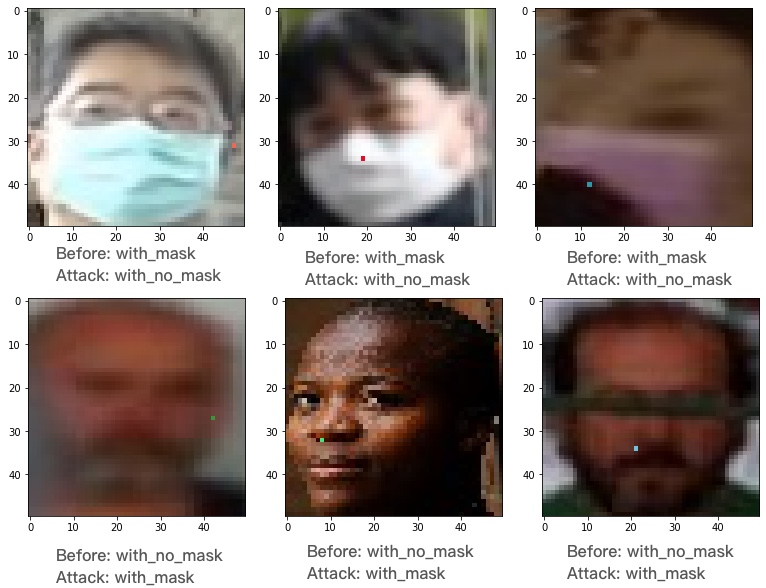
\includegraphics[width=8cm]{Slice.jpg}
    \caption{Selected Examples of Successful Attacks.}
\end{figure}

\section{Conclusion}
In conclusion, our research trained a model with 94.20\% of accuracy on determine whether a face wear the mask or not. Then our further investigation on reveal the feasibility of one pixel attack, but due to structure of the face mask detection model, the success rate of attack is limited. For future research, we may focus on two kinds of improvements: performance and accuracy of attack. The model now requires about 10 seconds to process a image which is far from real-time detection. The MTCNN is the bottleneck, and we may replace MTCNN with our own model for future research. Similarly, we can work on better algorithm in future research to achieve higher success rate in one pixel attacks.

\section{Significance}
The final result of 94.20\% accurracy has proved that the automatic mask detection could be achieved by using the ResNet model. Moreover, this automatic mask detection system could correctly distinguish between regular and surgical masks. This study's finding will rebound social benefits during a pandemic period. Wearing a mask is crucial, because it could prevent respiratory droplets, which is often a vehicle for viral transmission, reaching other people. Therefore, This automatic mask detection could be used in public space, such as shopping malls, supermarkets, hospitals. For the government, This system could check people if they are wearing correct masks so that it could directly enhance the implementation of epidemic prevention policy. For the business owners, this high efficiency mask detection could reduce the workload due to manual operation, so the running cost will be reduced clearly. Overall, this mask detection system could bring multiple positive effects to the current society. 



\begin{thebibliography}{9}
\bibitem{tshirt}
Lee, Alex. \textit{This ugly t-shirt makes you invisible to facial recognition tech.} {\em Wired}, https://www.wired.co.uk/article/facial-recognition-t-shirt-block. 
\bibitem{github}
    Kondratyuk, Dan. https://github.com/Hyperparticle/one-pixel-attack-keras.

\bibitem{onepixel}
    Su, jiawei et al.  \textit{One pixel attack for fooling deep neural networks.}, {\em IEEE Transactions on Evolutionary Computation}, Vol.23 , Issue.5 , pp. 828--841. https://arxiv.org/abs/1710.08864.
    
\bibitem{kaggle}
    Wobot Intelligence. \textit{Face Mask Detection Dataset.}, {\em Kaggle Co.}, https://www.kaggle.com/wobotintelligence/face-mask-detection-dataset.
    
\bibitem{facemaskdetect}
    Nagrath, P., Jain, R., Madan, A., Arora, R., Kataria, P., \& Hemanth, J. (2021). SSDMNV2: A real time DNN-based face mask detection system using single shot multibox detector and MobileNetV2. Sustainable cities and society, 66, 102692.

\bibitem{Yolo-v2}
    Loey, M., Manogaran, G., Taha, M. H. N., \& Khalifa, N. E. M. (2021). Fighting against COVID-19: A novel deep learning model based on YOLO-v2 with ResNet-50 for medical face mask detection. Sustainable cities and society, 65, 102600.


\end{thebibliography}



\end{document}
